% !TeX root = ../mde-presentation.tex

\section{2-Minute Madness} \label{sec:madness}
%%%%%%%%%%%%%%%%   TITLE PAGE   %%%%%%%%%%%%%%%%%%
\subsection*{Title page}  % to show it in the title bar

\begin{frame}
	\frametitle[MDE title page]{}
	\vspace{2.0cm}
	\begin{center}
		{\color{black}
			\textbf{
				\fontsize{36pt}{38pt}\selectfont \presentationtitle\\
				\vspace{1.5cm}}}
		\textbf{
			\fontsize{26pt}{28pt}\selectfont \presentationsubtitle \\
		}
		\vspace{1.5cm}
		{\fontsize{18pt}{20pt}\selectfont
			\location, \presentationdate \\
			\vspace{1ex}
			\hyperlink{frm:author}{\presentationauthor} \\
			\vspace{1.5cm}
			\textit{
				Helmholtz Coastal Data Center \\
				Helmholtz-Zentrum Hereon
		}}

	\end{center}

    \begin{textblock*}{6cm}(0.05\textwidth,0.95\textheight)
        \href{https://hcdc.hereon.de}{
\includegraphics[width=6cm]{figures/hcdc.pdf}}
    \end{textblock*}

    \begin{textblock*}{6cm}(0.8\textwidth,0.95\textheight)
        \hyperlink{frm:map}{
\includegraphics[width=6cm]{figures/hereon.png}}
    \end{textblock*}

\end{frame}

\subsection*{Core features}

\begin{frame}{A central platform to access Model Data}
    \begin{block}{Core features}
        \begin{columns}
            \begin{column}{0.5\textwidth}
                \begin{itemize}
                    \item View 4D Model-Data on a map
                    \item Categorized: One page per project, institution,
                        author, etc. with all corresponding model runs
                    \item Search and filter model runs and groups
                    \item Compute and compare statistics on/of subsets of
                        Model Data
                    \item Download the raw data for the selected region
                \end{itemize}
            \end{column}
            \begin{column}{0.5\textwidth}
                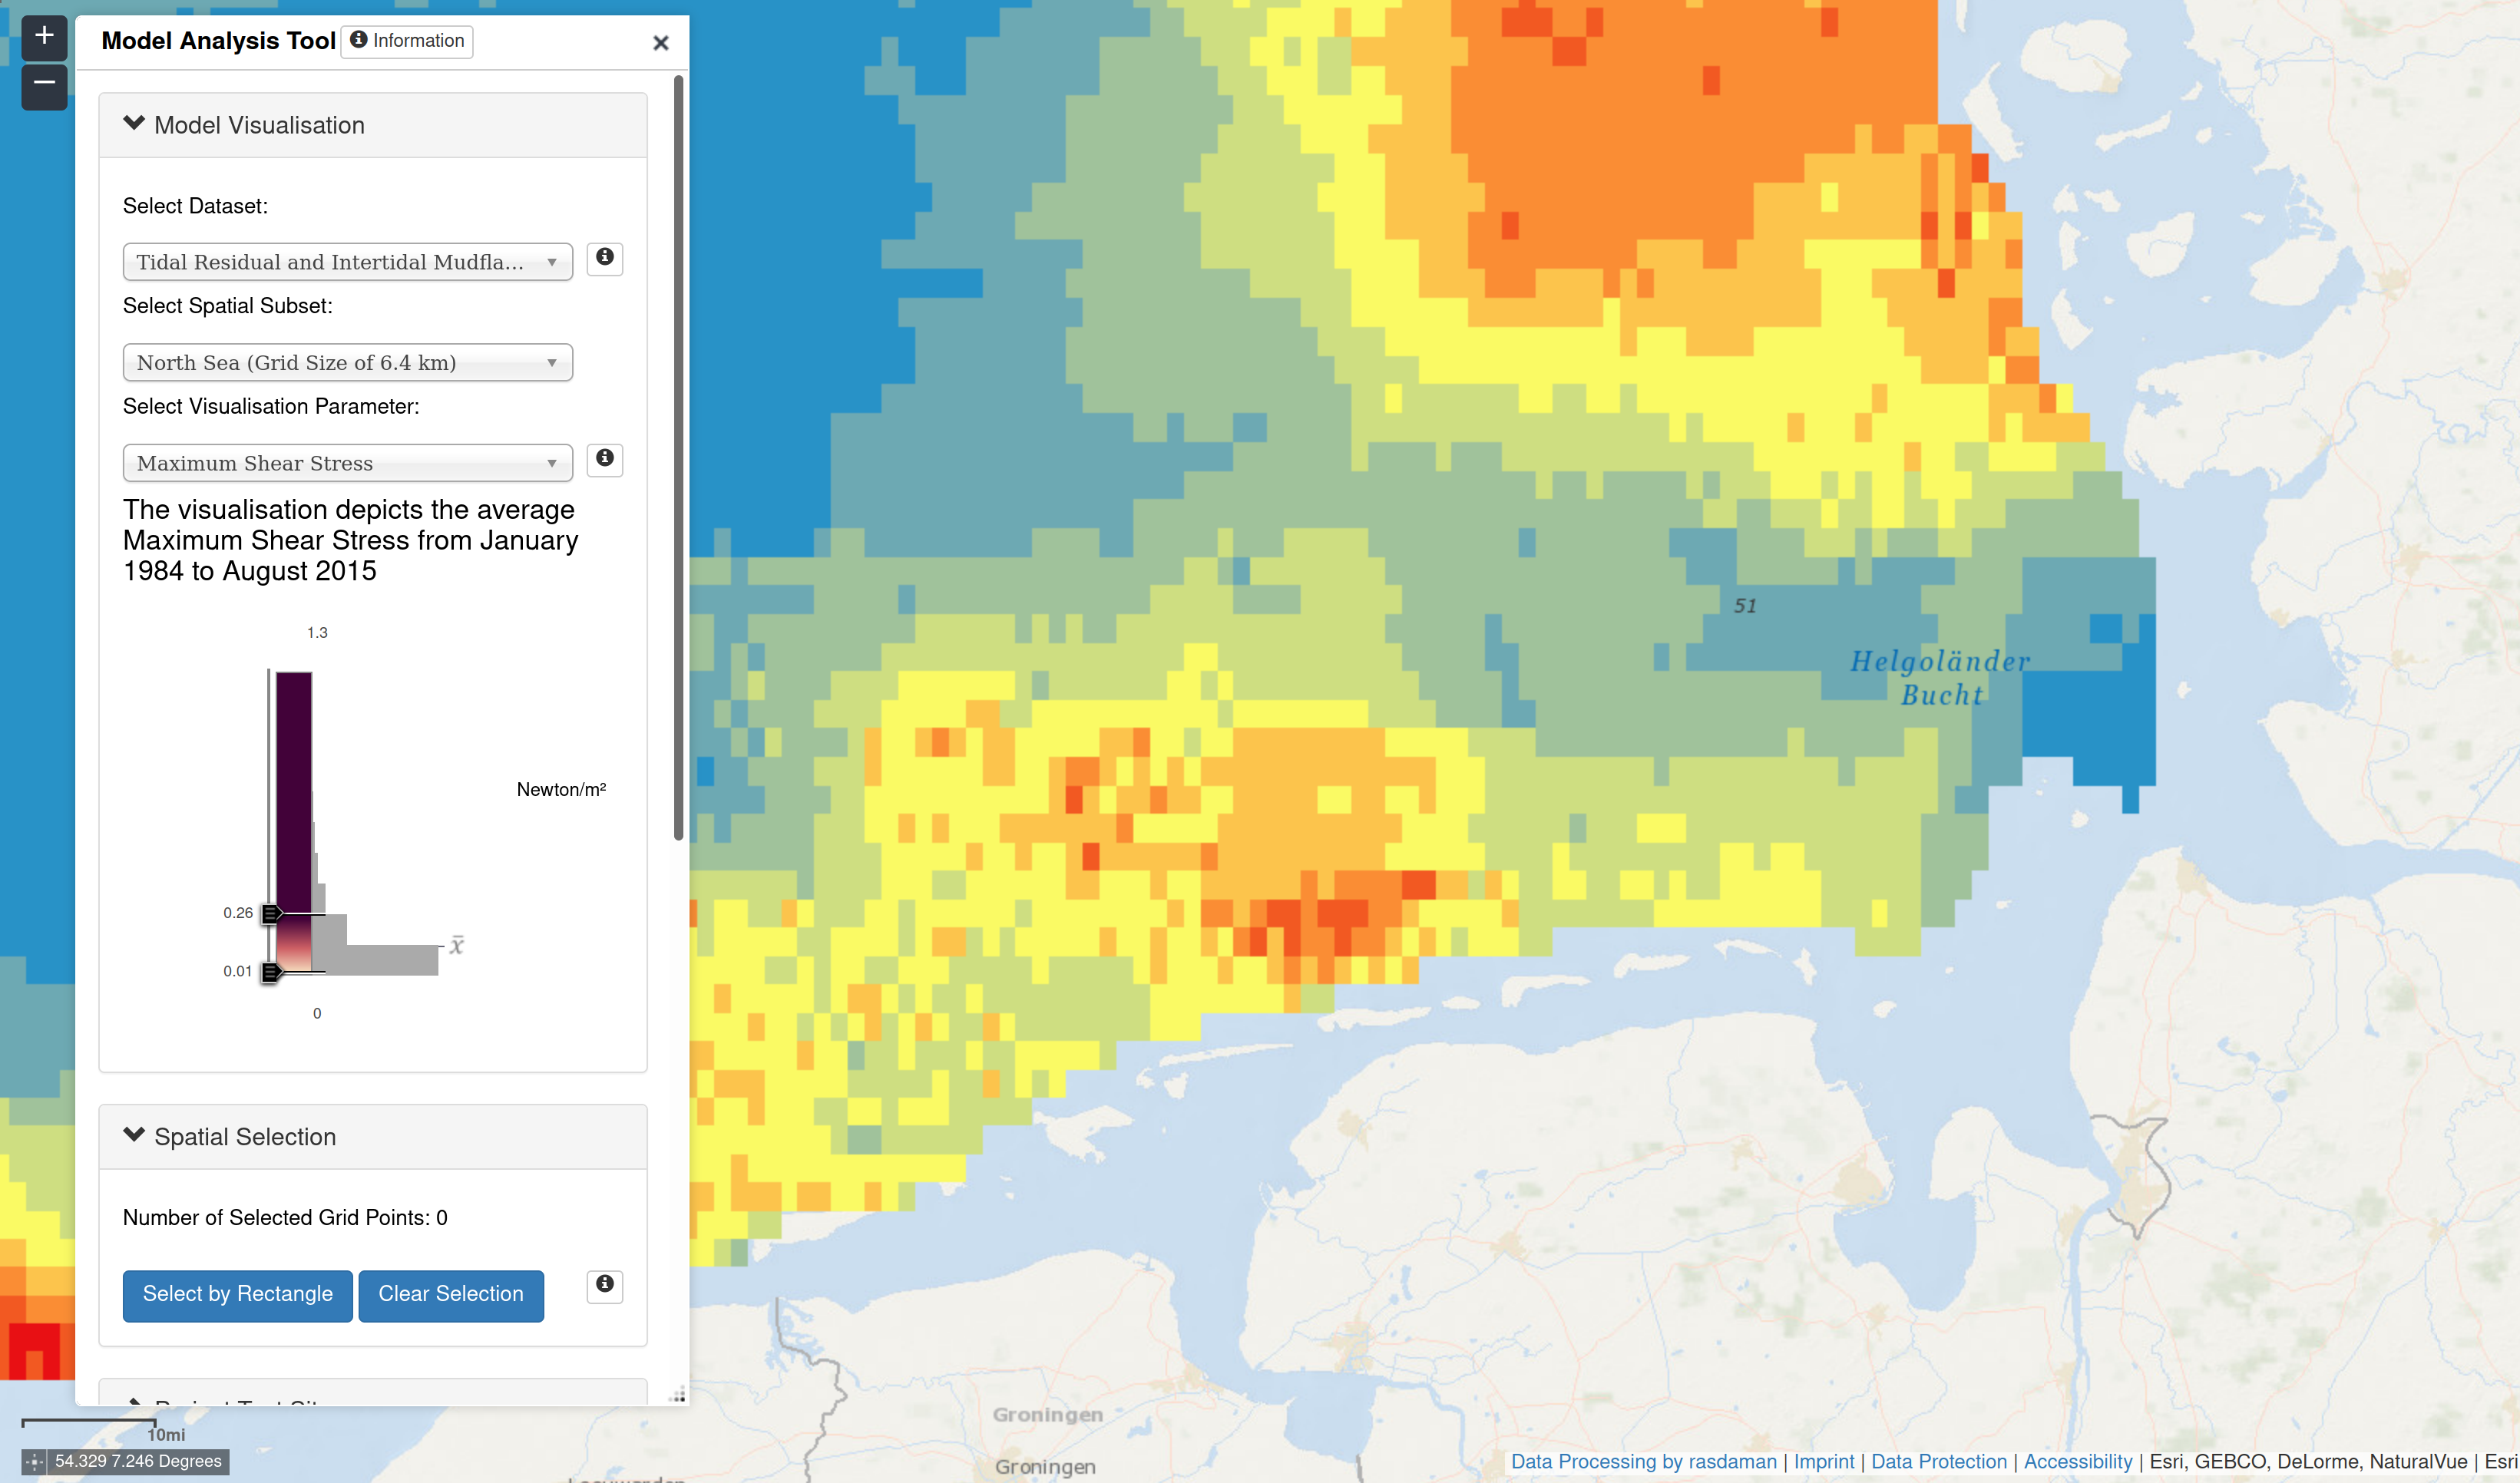
\includegraphics[width=\textwidth]{figures/demo-screenshot-model-data-explorer.png}
            \end{column}
        \end{columns}
    \end{block}
\end{frame}

\subsection*{Service Plugins}

\begin{frame}{A modular and federated system}
    \begin{columns}
        \begin{column}{0.3\textwidth}
            \begin{itemize}
                \item Single configuration interface for multiple connected
                    services
                \item multiple standard interfaces
                \item Federation to connect multiple research centers
            \end{itemize}

            \vspace{1em}

            \hyperlink{frm:service-plugins}{\beamerbutton{\normalsize More \ldots}}
        \end{column}
        \begin{column}{0.7\textwidth}
            \includegraphics[width=\textwidth, page=2]{figures/mde-service-plugins-basic.pdf}
        \end{column}
    \end{columns}
\end{frame}